\chapter{Evaluation} \label{sec:evaluation}

\section{Environment}

All the code has been run on the \enquote{Astral} high performance computer of Cranfield's university. The operating system is SUSE Linux Enterprise Server 11 (64 bits architecture), with a Linux 3 kernel.

The system is separated in login nodes and compute nodes. There are two \enquote{front-end} login nodes and they contain two Intel E5-2660 (Sandy Bridge - 8 cores) CPUs giving 16 CPU cores and have a total of 192 GB of shared memory. The login nodes enable the user to connect to the system and compile one's program. There are 80 compute nodes, each node having two Intel E5-2660 (Sandy Bridge - 8 cores) CPUs. This is giving a total of 1280 available cores. Each compute node have at least accessed to 64 GB shared memory. Nodes are connected with Infiniband\TM low-latency interconnect.

\section{Segmentation metrics}

To measure the precision of the localisation / segmentation algorithm, we use the metrics as defined in \cite{pascalVoc2012} \footnote{Information on the evaluation system can be found at  \url{http://host.robots.ox.ac.uk/pascal/VOC/voc2012/devkit_doc.pdf}}.

To be considered a correct detection, the \textbf{Intersection over Union} $IoU$ between the predicted bounding box $B_p$ and ground truth bounding box $B_{gt}$ must exceed 50\% by the formula:

$$IoU = \frac{area(B_p \cap B_{gt})}{area(B_p \cup B_{gt})}$$

To simplify the calculation, this formula can be rewritten as:

$$IoU = \frac{area(B_p \cap B_{gt})}{area(B_p) + area(B_{gt}) - area(B_p \cap B_{gt})} $$

Using this metric, we can compute the precision $P$, the recall $R$ and the accuracy $A$ given by:

$$ P =  \frac{T_p}{T_p + F_p}$$
$$ R =  \frac{T_p}{T_p + F_n}$$
$$ A = \frac{T_p}{T_p + F_n + F_p} $$

with:
\begin{itemize}
   \item $T_p$ the number of true positives (the bounding boxes correctly localised)
   \item $F_p$ the number of false positives (the predicted bounding boxes incorrectly localized)
   \item $F_n$ the number of false negative (the ground truth bounding boxes not localized)
\end{itemize}

Note that given the convention from \cite{pascalVoc2012}, if more than one predicted bounding box overlaps the same ground truth bounding box, only one will be considered as $T_P$, the rest will be $F_P$s.

\section{Cross validation}

Cross validation is a technique used to assert the generalization to a new dataset of the different metrics used. 

A common type of cross validation is the k-fold cross validation. In this method, the original sample is randomly split into $k$ partitions of equal sized. Of these generated subsamples, a single split is used for test set, the remaining are used as training data.
This last task is repeated $k$ times, each of the k partitions being used only once for testing. The $k$ results can then be averaged to produce a single estimation (illustrated in figure  \ref{fig:4-fold_cross_validation})

The advantage of this method over repeated random sub-sampling is that all observations are used for both training and testing, each observation being used for testing exactly once. 

10-fold cross-validation were used for all the presented results (the most common fold value that maximises the training set size).

\begin{figure}[h]
    \tikzset{myshade/.style={minimum size=.5cm, outer color ={#1!90!gray}, inner color={#1!90!gray}}}
    \newcommand\myrect[1][]{\tikz\node[rectangle,myshade=#1]{};}
    
    \centering
    \begin{tabular}{rccccl}
        First iteration & \myrect[orange] & \myrect[blue] & \myrect[blue] & \myrect[blue] &\\
        Second iteration & \myrect[blue] & \myrect[orange] & \myrect[blue] & \myrect[blue] & \hspace{1cm} \myrect[blue] : Fold for training \\
        Third iteration & \myrect[blue] & \myrect[blue] & \myrect[orange] & \myrect[blue] & \hspace{1cm} \myrect[orange] : Fold for testing \\
        Fourth iteration & \myrect[blue] & \myrect[blue] & \myrect[blue] & \myrect[orange] &\\
    \end{tabular}
    \caption{Illustration of 4-fold cross validation}
    \label{fig:4-fold_cross_validation}
\end{figure}

\section{Results}

First, the localisation and classification processes were run independently (using the ground truth bounding box for classification).

\subsection{Localisation}

\begin{table}[h]
    \centering
    \renewcommand{\arraystretch}{1.2}
    \begin{tabular}{|c | c c|} 
        \hline
        Metric (average) & My method & DCNN from \cite{Bolanos2016} \\
        \hline
        Accuracy & \textbf{74\%} & 60\% \\ 
        \hline
        Recall &  \textbf{74\%} & 80\% \\
        \hline
        Precision &  \textbf{79\%} & 70\% \\
        \hline
    \end{tabular}
    \caption{Average localisation accuracy result for UEC FOOD 256}
    \label{table:localisation_result}
\end{table}

The table \ref{table:localisation_result} gathers the average accuracy, recall, precision of my localisation method using a DCNN pre-trained on salient object detection. In \cite{Bolanos2016}, Bolanos use a fine-tuned pre-trained Deep Neural Network and obtain around 60\% of accuracy (using the same IoU over 50\%). It was fine-tuned to detect bounding boxes containing food on multiple datasets.

Compare to the found literature, my method lead to a higher accuracy. It seems that the assumptions made to switch from a DCNN trained to detect food / non-food detection to salient object detection is founded. Moreover, a higher accuracy is not to the detriment of the recall or precision.

For the result of the table \ref{table:localisation_result}, we use an IoU of 50\%. In Fig \ref{fig:segmentation_overlap}, we can see that the metrics' values are greatly influenced by the threshold choose for correctness (from 73\% of average accuracy with a threshold at 50\% to 0\% of accuracy for a threshold of 100\%).

\begin{figure}
    \centering
    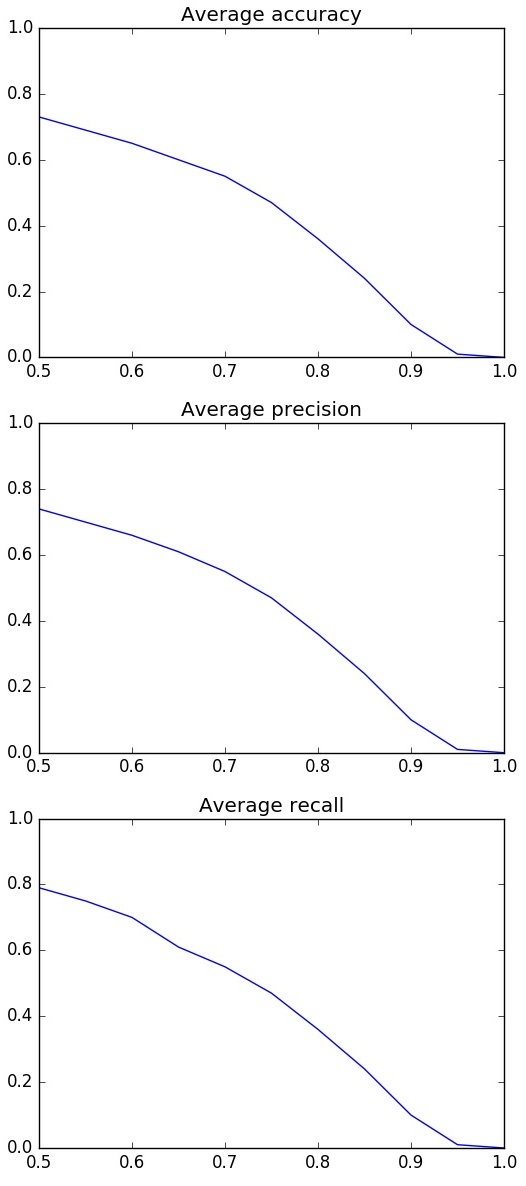
\includegraphics[scale=0.5]{img/segmentation_overlap.jpg}
    \caption{Curves of Accuracy over IoU (top), Precision over IoU (centre) and Recall over IoU (bottom)}
    \label{fig:segmentation_overlap}
\end{figure}

\subsection{Classification}

\begin{table}
    \centering
    \renewcommand{\arraystretch}{1.2}
    \begin{tabulary}{\textwidth}{| c | C|}
        \hline
        Method & Average accuracy \\
        \hline
        CNN as descriptor + RF & \textbf{40\%} \\ 
        \hline
        BoW (1000 words)+ SVM with $\chi^2$ & 10\% \\ % made up!
        \hline
        LBP + CHM + Decision tree & 5\% \\ 
        \hline
        LBP + CHM + SVM & 11\% \\ % made up!
        \hline
        LBP + CHM + RF & 16\% \\ % improved!
        \hline
        DCNN from \cite{Bolanos2016} & 63\%\\
        \hline 
        DCNN from \cite{Yanai2015} & 67\%\\
        \hline 
    \end{tabulary}
    \caption[Average classification accuracy result for UEC FOOD 256]{Average classification accuracy result for UEC FOOD 256. CHM stands for colour histograms and moments}
\end{table}

In \cite{Bolanos2016}, the authors use a fine-tuned pre-trained Deep Neural Network and obtain 63\% accuracy on UEC FOOD-256.

In \cite{Yanai2015}, the authors use a fine-tuned pre-trained Deep Neural Network and obtain 67\% accuracy on UEC FOOD-256.


\subsection{Localisation and classification}

Using the segmentation and classification method with the highest accuracy, i.e. saliency detection DCNN segmenter with DCNN as a feature descriptor and random forest classifier, we present the final results fixing the IoU threshold to 50\% in table \ref{table:uecfood100_results}. The total accuracy is 28\% that is 9 points below the method presented by Bolanos et al. in 2016 \cite{Bolanos2016}. The localisation process is able to find most of the items in a picture.

\begin{table}
    \centering
    \renewcommand{\arraystretch}{1.2}
    \begin{tabulary}{\textwidth}{| c | C C|}
        \hline
        Process & My method & DCNN from \cite{Bolanos2016} \\
        \hline
        Overall & \textbf{28\%} & 37\% \\ 
        \hline
        Localisation &  \textbf{74\%} & 60\% \\
        \hline
        Classification &  \textbf{38\%} & 60\% \\
        \hline
    \end{tabulary}
    \caption{Average accuracy result for simultaneous localisation and recognition on UEC-FOOD 256}
    \label{table:uecfodd256_results}
\end{table}

\begin{figure}
    \centering
    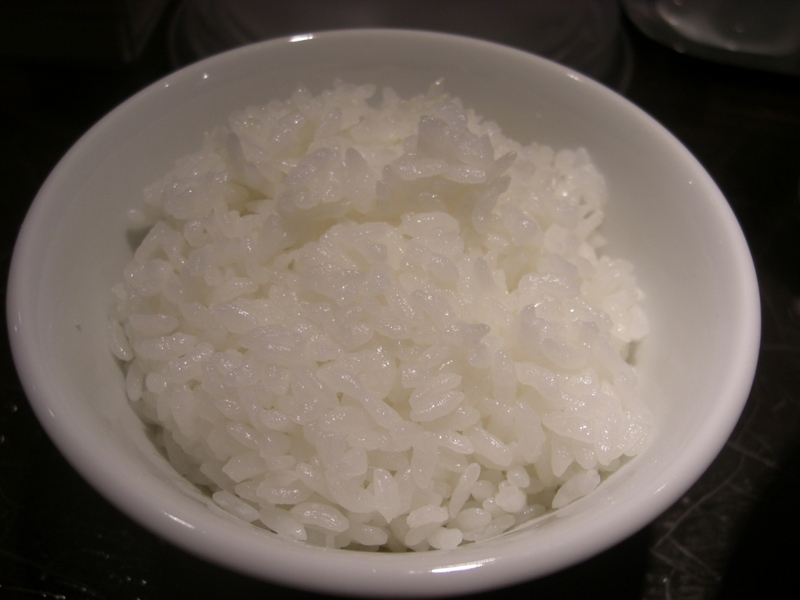
\includegraphics[height=2.5cm, width=2.5cm]{img/top_rice.jpg}
    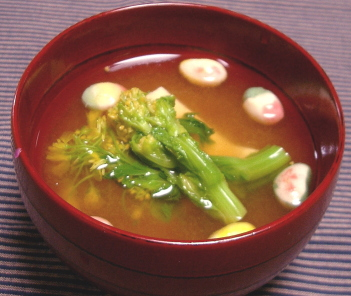
\includegraphics[height=2.5cm, width=2.5cm]{img/top_miso_soup.jpg}
    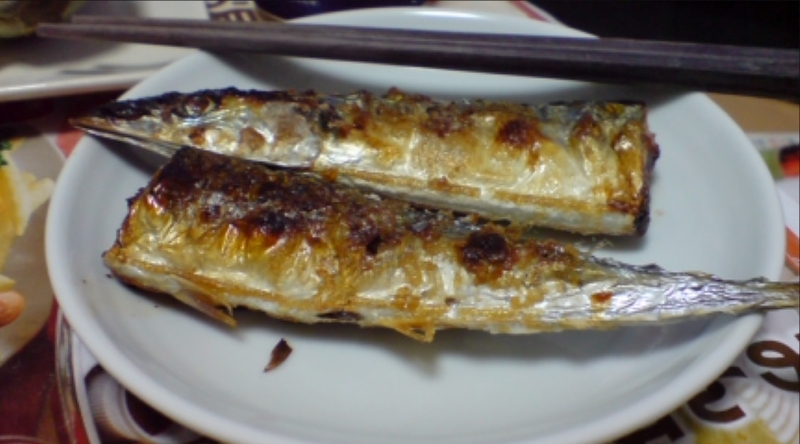
\includegraphics[height=2.5cm, width=2.5cm]{img/top_grilled_pacific_saury.jpg}
    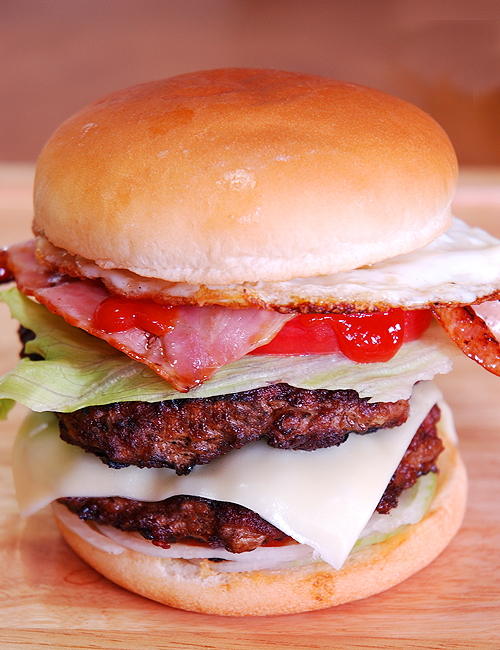
\includegraphics[height=2.5cm, width=2.5cm]{img/top_hamburger.jpg}
    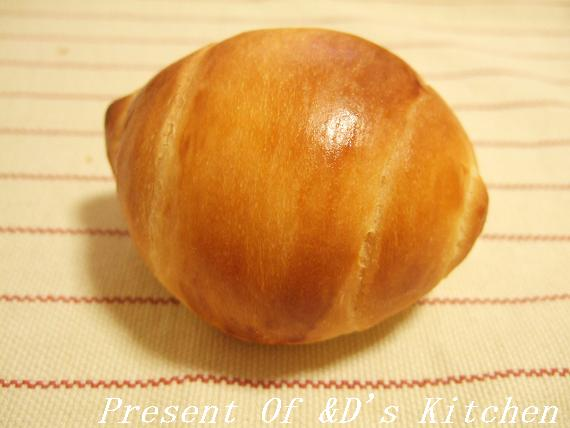
\includegraphics[height=2.5cm, width=2.5cm]{img/top_roll_bread.jpg}
    \caption[Classes having the highest accuracy]{The five classes having the highest accuracy with (from the left to the right, starting from the highest accuracy) rice (98\%), miso soup (95\%), grilles pacific saury (94\%), hamburger (93\%), roll bread (90\%)}
    \label{fig:top_5}
\end{figure}

As can been seen in Fig \ref{fig:top_5} and \ref{fig:least_5}, the best performing class is rice and the least one is tanmen. The possible explanations are:
\begin{itemize}
    \item rice is the most represented food items in the dataset, maximising the size of the training sets (same for miso soup)
    \item rice has a specific texture and colour that is relatively invariant to the condition
    \item tanmen is a soup containing noodle and various vegetables. Thus, it can occur in different colour, shape and size.
    \item there are numerous soups in the dataset and tanmen is often confused with them. Figure \ref{fig:confusing_4} show the most class couples that are the most confused and it shows that clear  and miso soup are often mixed up by the method.
\end{itemize}

%14 roll bread 0.905660291919
%17 hamburger 0.936073016618
%49 grilled pacific saury 0.941860410357
%1 rice 0.952117846186
%36 miso soup 0.974164118934

\begin{figure}
    \centering
    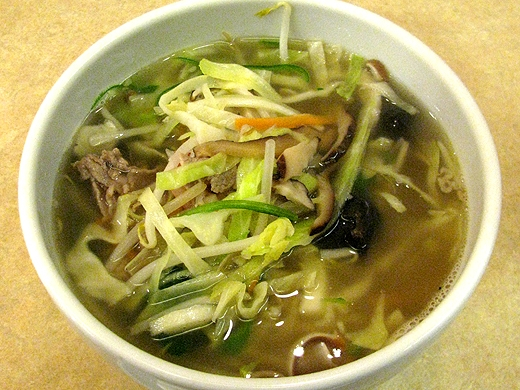
\includegraphics[height=2.5cm, width=2.5cm]{img/least_tanmen.jpg}
    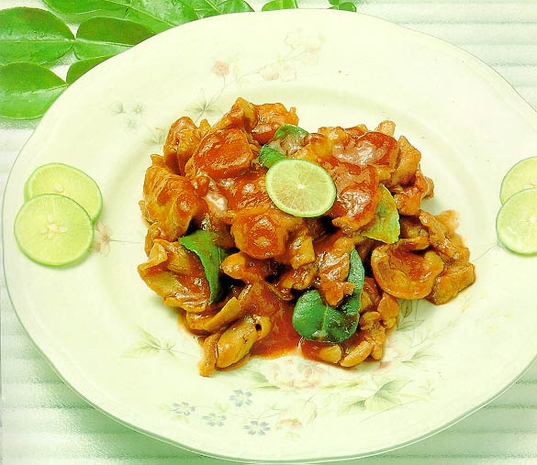
\includegraphics[height=2.5cm, width=2.5cm]{img/least_pork_with_lemon.jpg}
    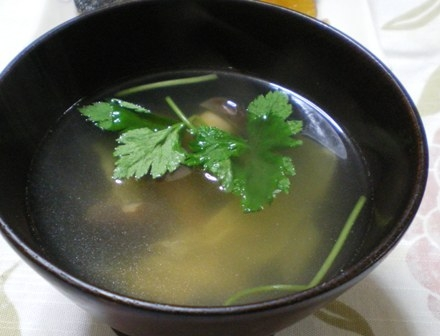
\includegraphics[height=2.5cm, width=2.5cm]{img/least_clear_soup.jpg}
    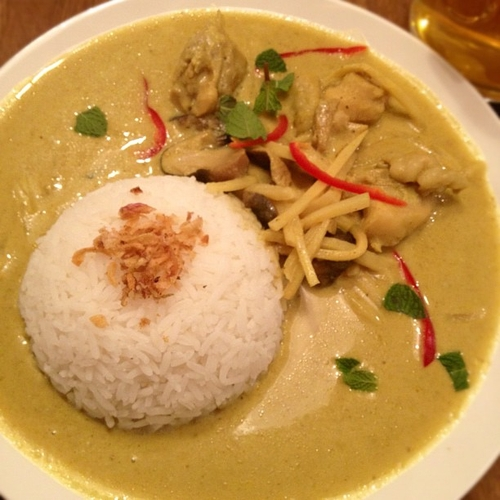
\includegraphics[height=2.5cm, width=2.5cm]{img/least_yellow_curry.jpg}
    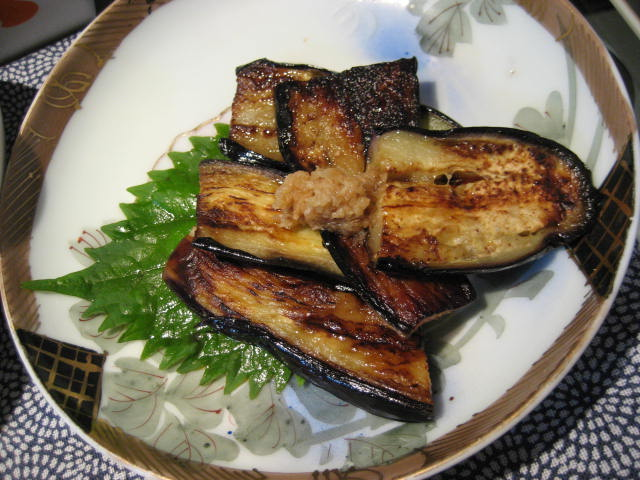
\includegraphics[height=2.5cm, width=2.5cm]{img/least_grilled_eggplant.jpg}
    \caption[Classes having the lowest accuracy]{The five classes having the lowest accuracy with (from the left to the right, starting from the lowest accuracy) tanmen (0\%), Pork with lemon (0\%), clear soup (1\%), yellow curry (1\%), grilles eggplant (1\%)}
    \label{fig:least_5}
\end{figure}

%111 tanmen 0.0
%193 Pork with lemon 0.0
%135 clear soup 0.00952380861678
%113 yellow curry 0.0104166655816
%33 grilled eggplant 0.0105263146814

\begin{figure}
    \centering
    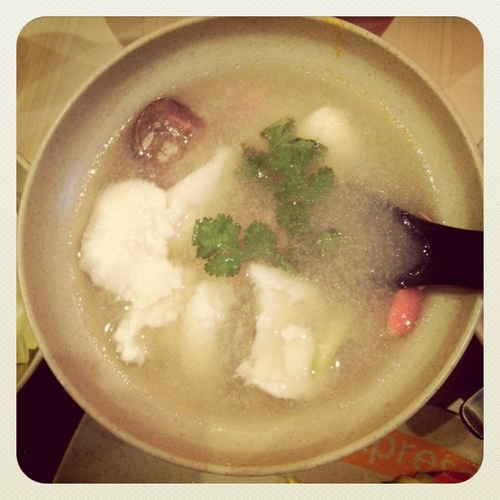
\includegraphics[height=5cm, width=5cm]{img/confusing_clear_soup.jpg}
    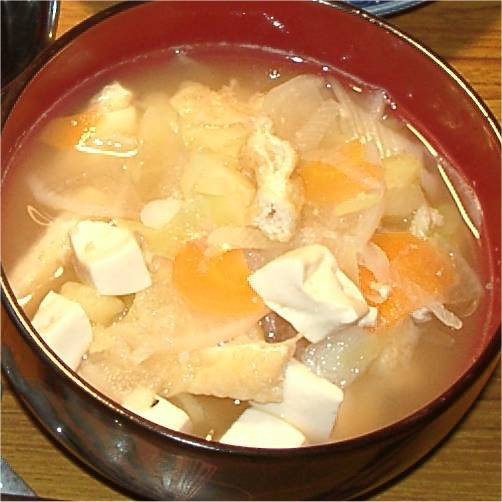
\includegraphics[height=5cm, width=5cm]{img/confusing_miso_soup.jpg}
    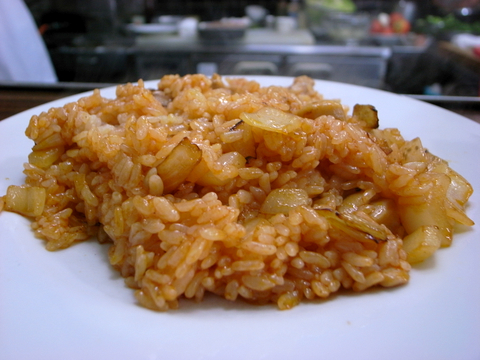
\includegraphics[height=5cm, width=5cm]{img/confusing_chicken_rice.jpg}
    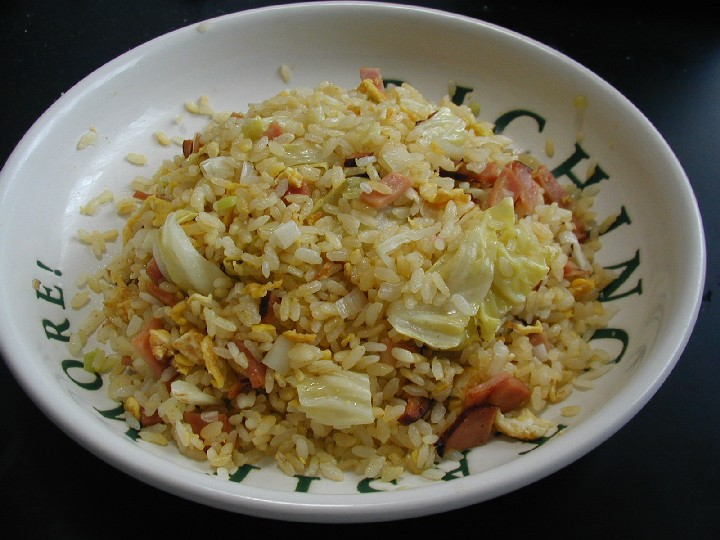
\includegraphics[height=5cm, width=5cm]{img/confusing_fried_rice.jpg}
    \caption[Most confused classes]{The four most confused classes (with from the left to the right, starting from the lowest accuracy) clear soup and miso soup (83\%), chicken rice and fried rice (54\%)}
    \label{fig:confusing_4}
\end{figure}

%134 35 clear soup || miso soup 0.838095158277
%88 35 Japanese tofu and vegetable chowder || miso soup 0.754716909932
%124 35 zoni || miso soup 0.727272661157
%156 35 oshiruko or red bean soup || miso soup 0.660194110661
%82 5 cutlet curry || beef curry 0.658914677604
%89 35 pork miso soup || miso soup 0.605504531605
%7 8 chicken rice || fried rice 0.460674105542
%23 22 beef noodle || ramen noodle 0.438596452755
%238 11 kaya toast || toast 0.43434339047
%135 35 yudofu || miso soup 0.431192620992

The method were also run the segmentation and classification on UEC FOOD 100. The results are presented in table \ref{table:uecfood100_results}. As UEC-FOOD 256, it can be seen that the localisation is better than the previous work with 67\% accuracy (the result is slightly lower than UEC-FOOD 256 as the dataset has a higher proportion of multiple food items per picture). The overall accuracy is 33\%.

\begin{table}
    \centering
    \renewcommand{\arraystretch}{1.2}
    \begin{tabulary}{\textwidth}{| C | C c c|} 
        \hline
        Process & My method & DCNN from \cite{Shimoda2015} & DCNN from  \cite{Kawano2014} \\
        \hline
        Overall & \textbf{33\%} & - & - \\ 
        \hline
        Localisation &  \textbf{67\%} & 60\% & - \\
        \hline
        Classification &  \textbf{50\%} & -  & 72\% \\
        \hline
    \end{tabulary}
    \caption{Average accuracy result for UEC FOOD 100}
    \label{table:uecfood100_results}
\end{table}
